% !TEX root = ../TUCthesis.tex
%****************************************************
\section{Implementierung}\label{ch:implementierung}
%****************************************************

% Schnittstellenrealisierung -> Interaktionsdiagramm
% Abfragen / Analysen:  "natürliche Sprache" + Code (evtl)

\subsection{Klassendiagramme}

%%%%%%%%%%%%%
%% Builder %%
%%%%%%%%%%%%%
\subsubsection{Builder.Builder}
Die Klasse \verb|Builder.Builder| hat die folgenden Schnittstellen:

\begin{figure}[H]
    \myfloatalign
    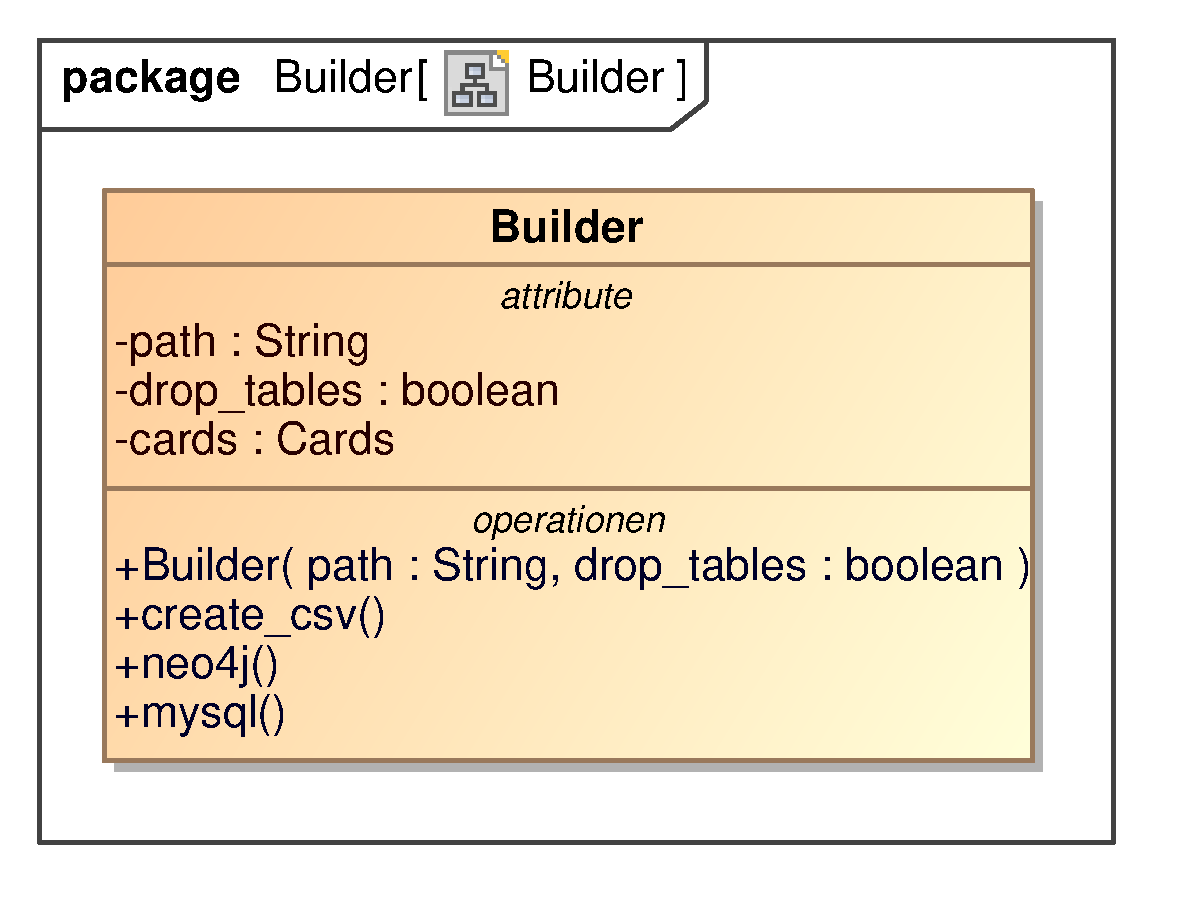
\includegraphics[width=0.75\textwidth]{gfx/MtGDeepAnalysis/Builder.eps}
    \caption{Klassendiagramm Builder.Builder}
    \label{fig:class:builder.builder}
\end{figure}

\begin{description}
    \item[constructor(path, drop\_tables)] \hfill \\
    Einrichten der Datenstruktur \verb|Cards| und speichern der übergebenen Argumente. Die Liste der Argumente befindet sich in \autoref{tab:builder.builder.constructor}
    \item[create\_csv()] \hfill \\
    Lädt die Kartendaten aus der \ac{JSON}-Datei und speichert die aufbereiteten Ergebnisse in \ac{CSV}-Dateien
    \item[neo4j()] \hfill \\
    Erstellt und befüllt die Neo4j Datenbank mit den Daten aus den \ac{CSV}-Dateien.
    \item[mysql()] \hfill \\
    Erstellt und befüllt die MySQL Datenbank mit den Daten aus den \ac{CSV}-Dateien.
\end{description}

\begin{table}[h]
    \caption{Builder.Builder::constructor(path : string, drop\_tables : boolean)} 
    \myfloatalign
    \begin{tabularx}{\textwidth}{lX}
        \toprule 
        \tableheadline{Eingabe} & \tableheadline{Beschreibung} \\ 
        \midrule 
        \verb|path : string| & Pfad zu der  \ac{JSON}-Datei, welche die Karten-Daten enthält \\
        \verb|drop_tables : boolean| & Angabe ob vor dem Einfügen der Daten in die Datenbank, alte Daten gelöscht werden sollen \\
        \bottomrule 
    \end{tabularx}
    \label{tab:builder.builder.constructor}
\end{table}


\subsubsection{Builder.Cards}
Die Klasse \verb|Builder.Cards| hat die folgenden Schnittstellen:

\begin{figure}[H]
    \myfloatalign
    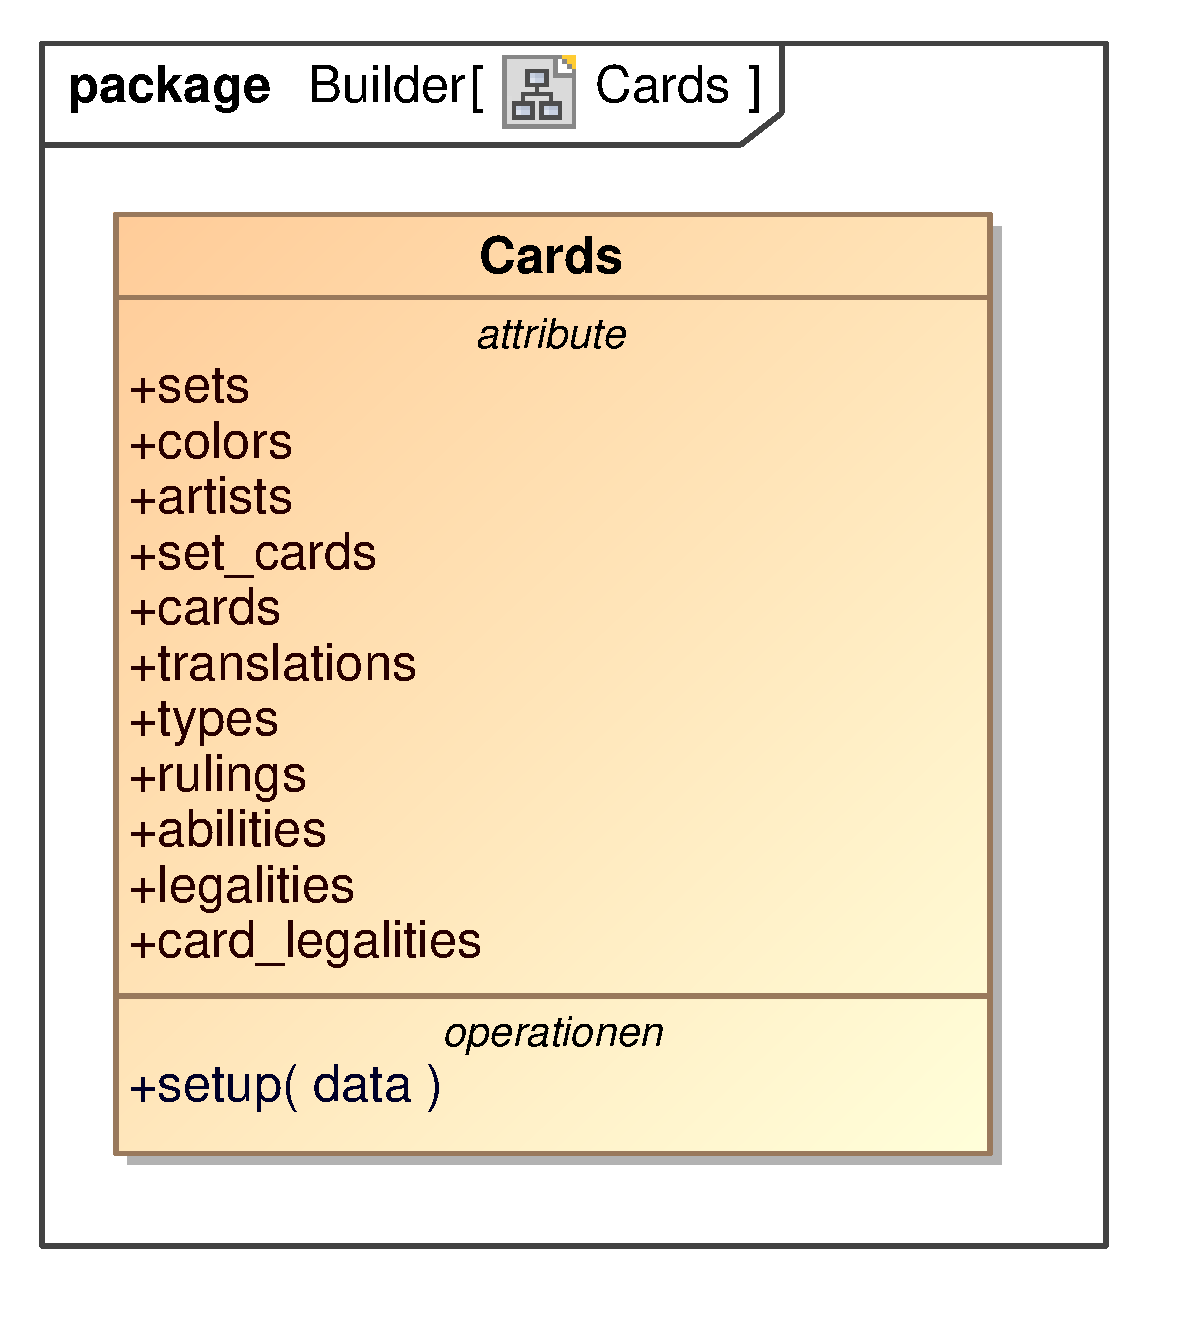
\includegraphics[width=0.75\textwidth]{gfx/MtGDeepAnalysis/Cards.eps}
    \caption{Klassendiagramm Builder.Cards}
    \label{fig:class:builder.cards}
\end{figure}

\begin{description}
    \item[constructor()] \hfill \\
    Erstelle Listen und Daten-Container.
    
    \item[setup(data)] \hfill \\
    Bearbeitet Kartendaten aus \ac{JSON}-Datei so, dass diese als \ac{JSON}-Dateien gespeichert werden können für den späteren Datenbank-Import. Die Liste der Argumente befindet sich in \autoref{tab:builder.cards}
   
\end{description}

\begin{table}[h]
    \caption{Builder.Cards::setup(data : Dictionary[])} 
    \myfloatalign
    \begin{tabularx}{\textwidth}{lX}
        \toprule 
        \tableheadline{Eingabe} & \tableheadline{Beschreibung} \\ 
        \midrule 
        \verb|data : Dictionary[]| & Liste mit allen Kartendaten die aufbereitet werden sollen \\
        \bottomrule 
    \end{tabularx}
    \label{tab:builder.cards}
\end{table}

\subsubsection{Builder.CSVHandler}
Die Klasse \verb|Builder.CSVHandler| hat die folgenden Schnittstellen:

\begin{figure}[H]
    \myfloatalign
    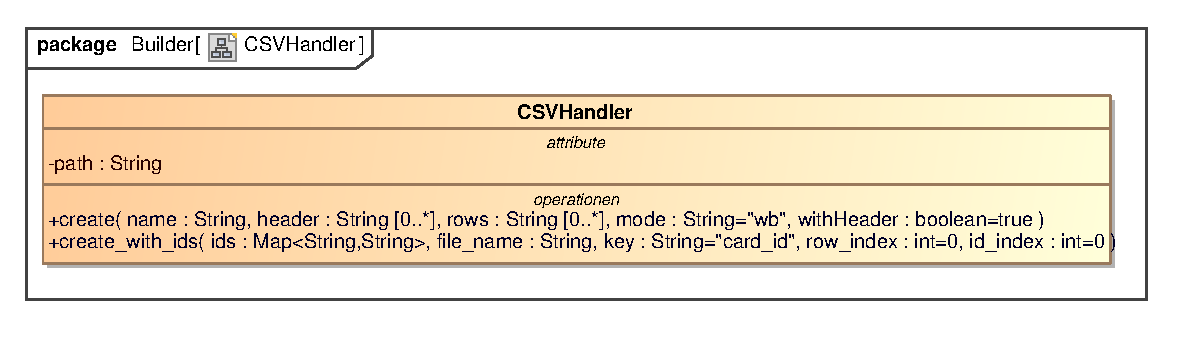
\includegraphics[width=\textwidth]{gfx/MtGDeepAnalysis/CSVHandler.eps}
    \caption{Klassendiagramm Builder.CSVHandler}
    \label{fig:class:builder.CSVHandler}
\end{figure}
%TODO: ...

\subsubsection{Builder.Tournaments}
Die Klasse \verb|Builder.Tournaments| hat die folgenden Schnittstellen:

\begin{figure}[H]
    \myfloatalign
    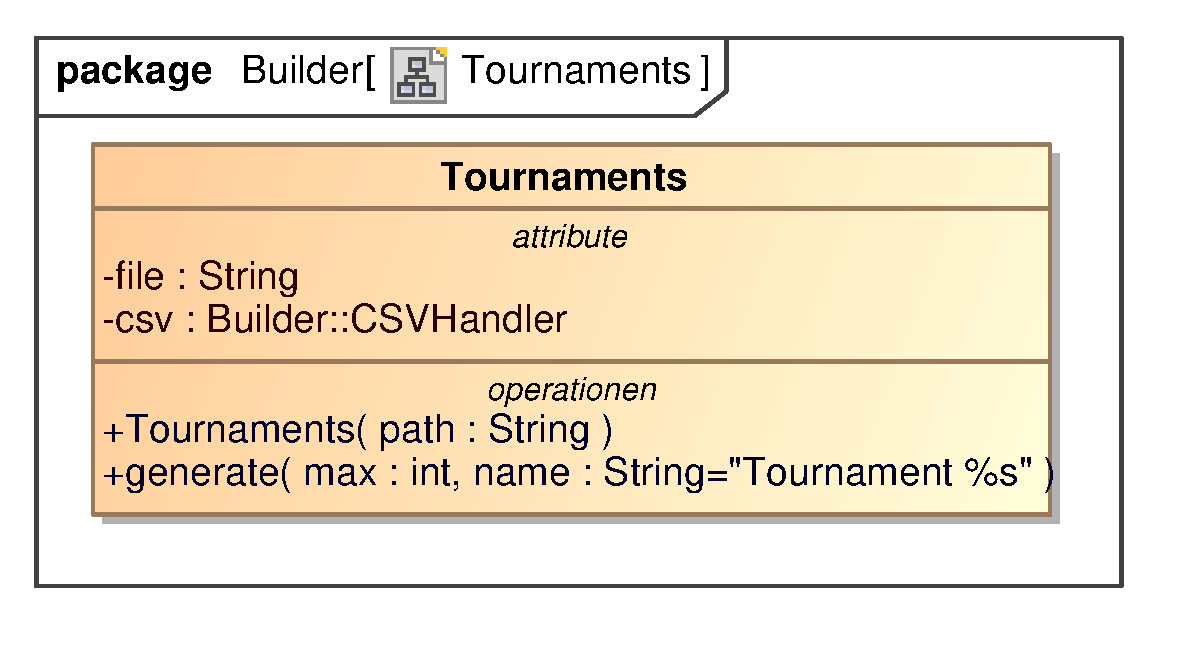
\includegraphics[width=0.75\textwidth]{gfx/MtGDeepAnalysis/Tournaments.eps}
    \caption{Klassendiagramm Builder.Tournaments}
    \label{fig:class:builder.Tournaments}
\end{figure}
%TODO: ...

%%%%%%%%%%%%%%%%%%%%%%
%% Builder.Handlers %%
%%%%%%%%%%%%%%%%%%%%%%
\subsubsection{Builder.Handlers.MySQLBuilder}
Die Klasse \verb|Builder.Handlers.MySQLBuilder| hat die folgenden Schnittstellen:

\begin{figure}[H]
    \myfloatalign
    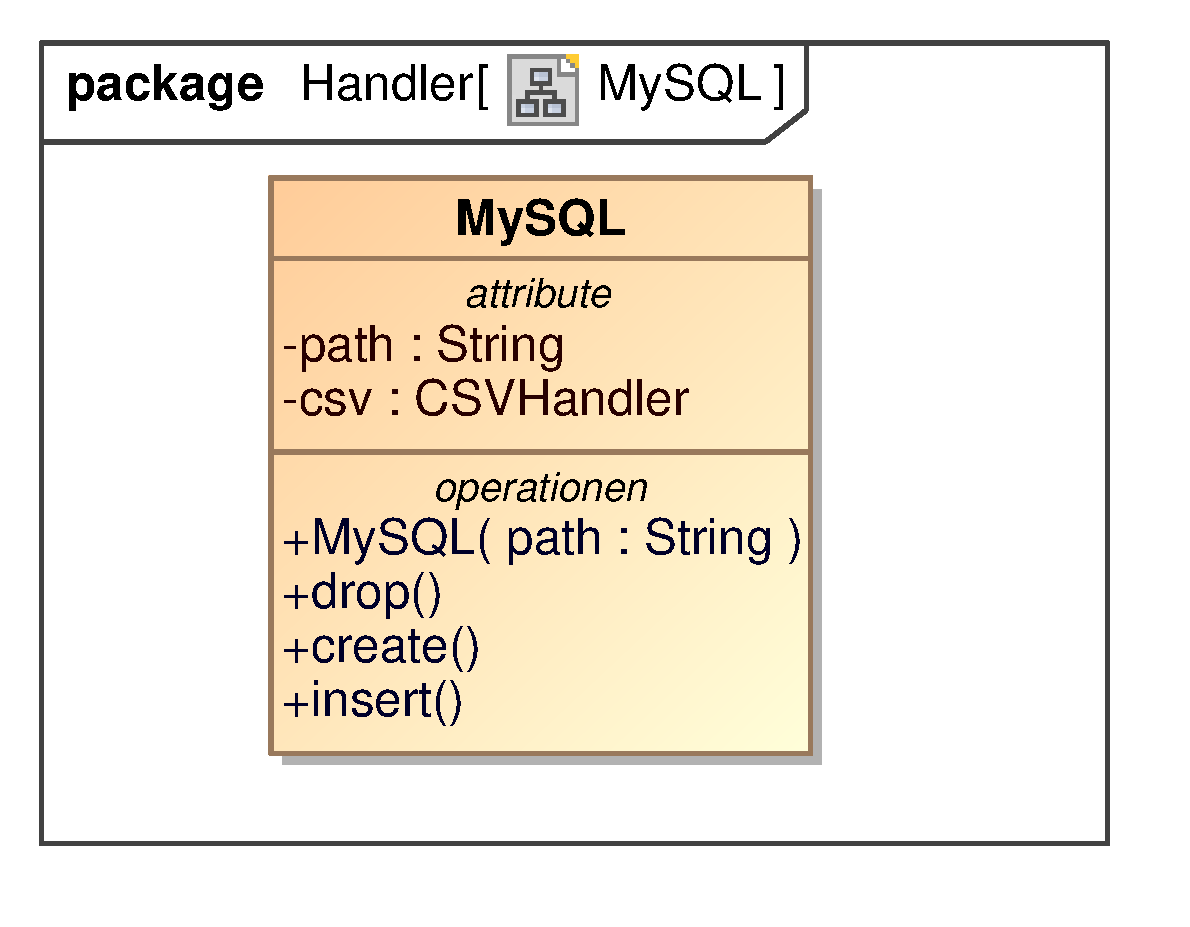
\includegraphics[width=0.75\textwidth]{gfx/MtGDeepAnalysis/MySQL.eps}
    \caption{Klassendiagramm Builder.Handlers.MySQLBuilder}
    \label{fig:class:builder.handlers.mysqlbuilder}
\end{figure}

\begin{description}
    \item[constructor(path)] \hfill \\
       Speichern der übergebenen Argumente. Die Liste der Argumente befindet sich in \autoref{tab:builder.handlers.mysqlbuilder.constructor}
    \item[drop()] \hfill \\
       Löscht Tabellen.
       
    \item[create()] \hfill \\
        Erstellt Tabellen.
        
    \item[insert()] \hfill \\
        Importiert Daten aus den \ac{CSV}-Dateien.
\end{description}

\begin{table}[h]
    \caption{Builder.Handlers.MySQLBuilder.constructor::setup(path : string)} 
    \myfloatalign
    \begin{tabularx}{\textwidth}{lX}
        \toprule 
        \tableheadline{Eingabe} & \tableheadline{Beschreibung} \\ 
        \midrule 
        \verb|path : string| & Pfad zu dem Verzeichnis welches die \ac{JSON} und \ac{CSV} Dateien enthält \\
        \bottomrule 
    \end{tabularx}
    \label{tab:builder.handlers.mysqlbuilder.constructor}
\end{table}


\subsubsection{Builder.Handlers.Neo4jBuilder}
Die Klasse \verb|Builder.Handlers.Neo4jBuilder| hat die folgenden Schnittstellen:

\begin{figure}[H]
    \myfloatalign
    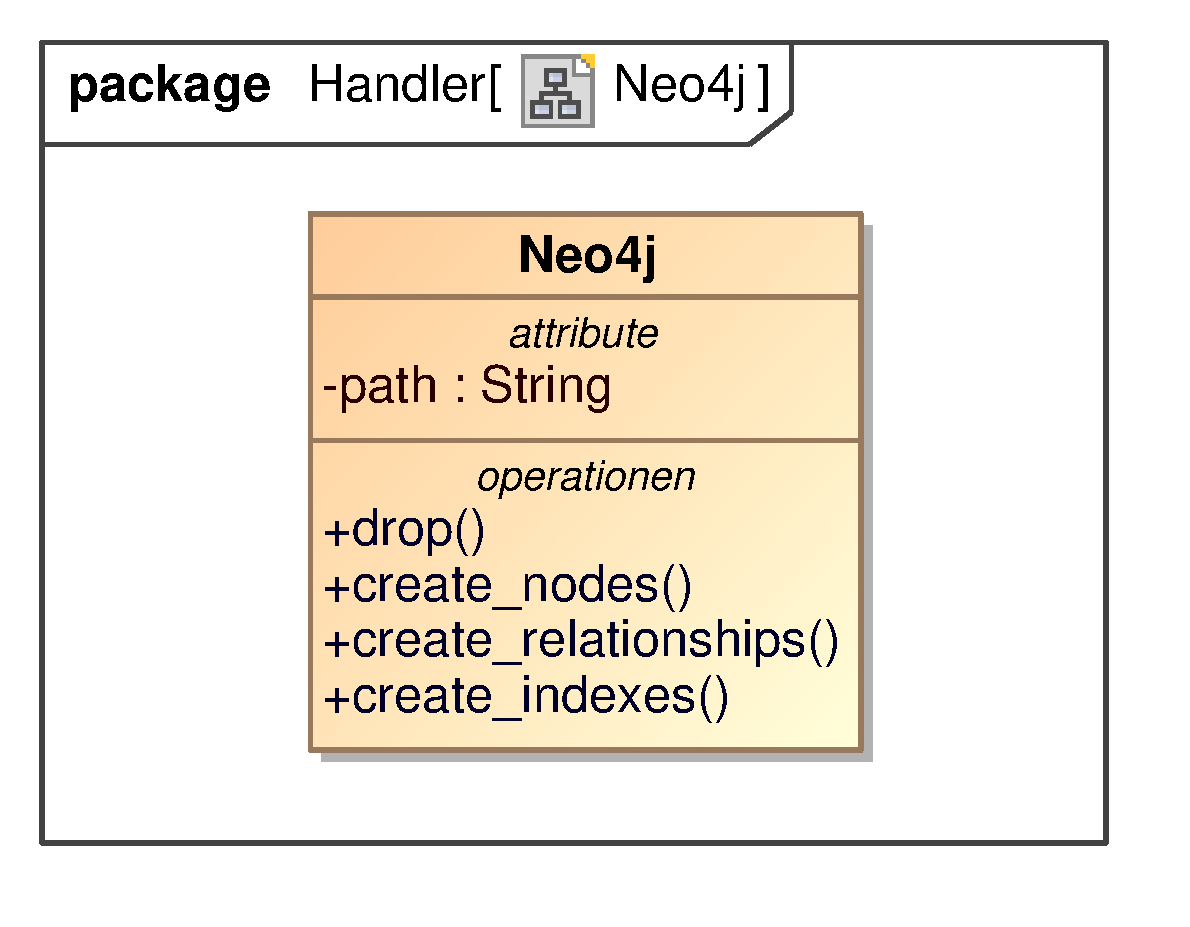
\includegraphics[width=0.75\textwidth]{gfx/MtGDeepAnalysis/Neo4j.eps}
    \caption{Klassendiagramm Builder.Handlers.Neo4jBuilder}
    \label{fig:class:builder.handlers.neo4jbuilder}
\end{figure}

\begin{description}
    \item[constructor(path)] \hfill \\
    Speichern der übergebenen Argumente. Die Liste der Argumente befindet sich in \autoref{tab:builder.handlers.neo4jbuilder.constructor}
    \item[drop()] \hfill \\
    Löscht Datenbank.
    
    \item[create\_nodes()] \hfill \\
    Erstellt alle Knoten mit Daten aus den \ac{CSV}-Dateien.
    
    \item[create\_indexes()] \hfill \\
    Erstellt Indizes.
    
    \item[create\_relationships()] \hfill \\
    Erstellen Beziehungen zwischen Daten aus den \ac{CSV}-Dateien.
\end{description}

\begin{table}[h]
    \caption{Builder.Handlers.Neo4jBuilder.constructor::setup(path : string)} 
    \myfloatalign
    \begin{tabularx}{\textwidth}{lX}
        \toprule 
        \tableheadline{Eingabe} & \tableheadline{Beschreibung} \\ 
        \midrule 
        \verb|path : string| & Pfad zu dem Verzeichnis welches die \ac{JSON} und \ac{CSV} Dateien enthält \\
        \bottomrule 
    \end{tabularx}
    \label{tab:builder.handlers.neo4jbuilder.constructor}
\end{table}


%%%%%%%%%%%%%%%%
%% Foundation %%
%%%%%%%%%%%%%%%%
\subsubsection{Foundation.Config}
Die Klasse \verb|Foundation.Config| hat die folgenden Schnittstellen:

\begin{figure}[H]
    \myfloatalign
    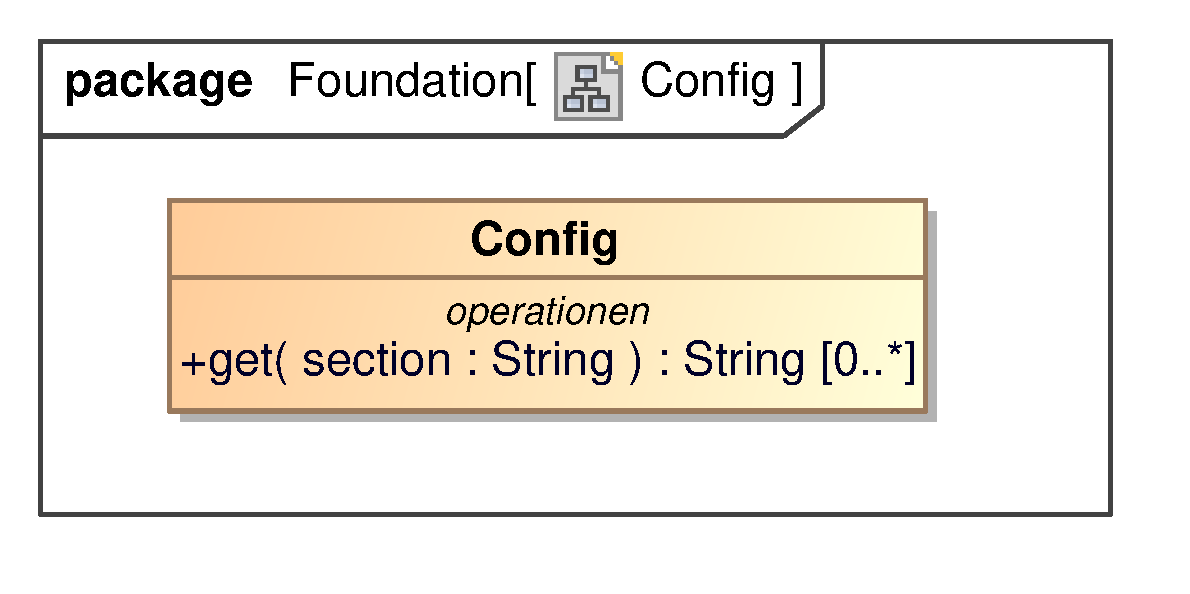
\includegraphics[width=0.75\textwidth]{gfx/MtGDeepAnalysis/Config.eps}
    \caption{Klassendiagramm Foundation.Config}
    \label{fig:class:foundation.config}
\end{figure}

\begin{description}
    \item[get(section)] \hfill \\
    Gibt einen Konfigurationsabschnitt aus der Datei \verb|config.ini| zurück. Die Liste der Argumente befindet sich in \autoref{tab:foundation.config.get}
\end{description}

\begin{table}[h]
    \caption{Foundation.Config::get(section : string) : string[]} 
    \myfloatalign
    \begin{tabularx}{\textwidth}{lX}
        \toprule 
        \tableheadline{Eingabe} & \tableheadline{Beschreibung} \\ 
        \midrule 
        \verb|section : string| & Name des Abschnitts der geladen werden soll \\
        \midrule  
        \midrule  
        \tableheadline{Ausgabe} & \tableheadline{Beschreibung} \\ 
        \midrule 
        \verb|string[]| & Konfigurationswerte des Abschnitts \\
        \bottomrule 
    \end{tabularx}
    \label{tab:foundation.config.get}
\end{table}


\subsubsection{Foundation.Database}
Die Klasse \verb|Foundation.Database| hat die folgenden Schnittstellen:

\begin{figure}[H]
    \myfloatalign
    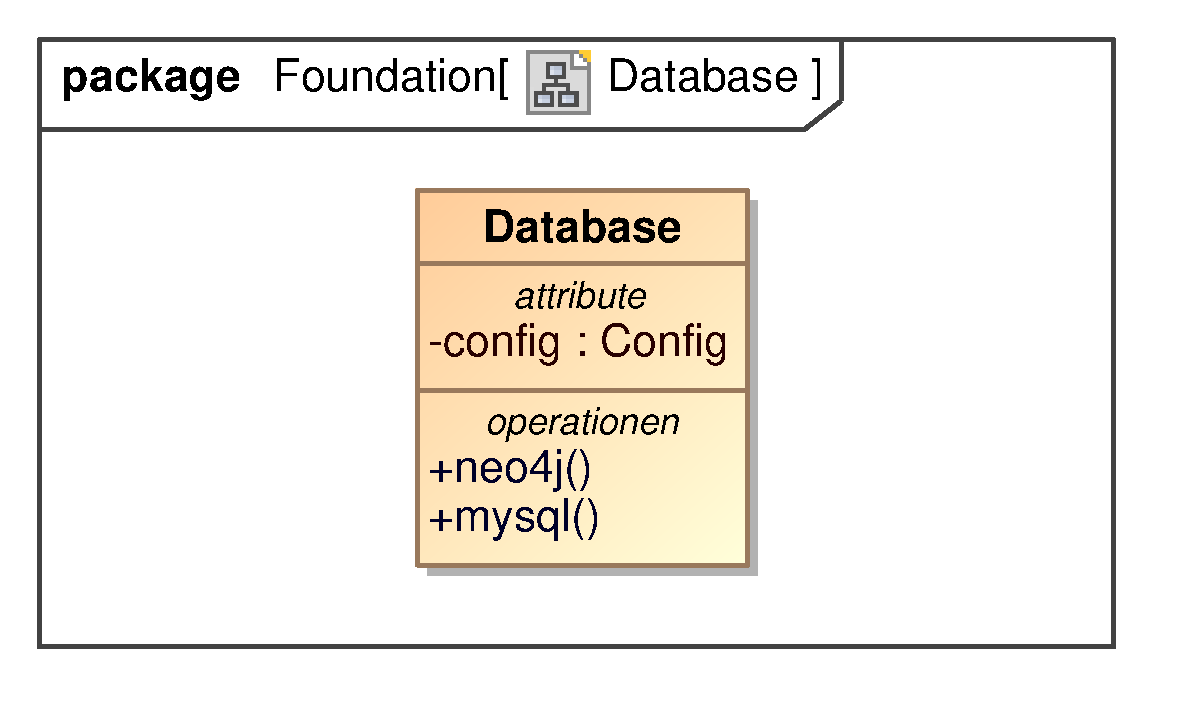
\includegraphics[width=0.75\textwidth]{gfx/MtGDeepAnalysis/Database.eps}
    \caption{Klassendiagramm Foundation.Database}
    \label{fig:class:foundation.database}
\end{figure}

\begin{description}
    \item[constructor()] \hfill \\
    Erstellt eine neue \verb|Foundation.Config| Instanz und speichert diese in \verb|config|.
    
    \item[neo4j()] \hfill \\
    Gibt eine neue Neo4j Datenbank-Instanz zurück.
    
    \item[mysql()] \hfill \\
    Gibt eine neue Mysql Datenbank-Instanz zurück.
\end{description}

\subsubsection{Foundation.Profiler}
Die Klasse \verb|Foundation.Profiler| hat die folgenden Schnittstellen:

\begin{figure}[H]
    \myfloatalign
    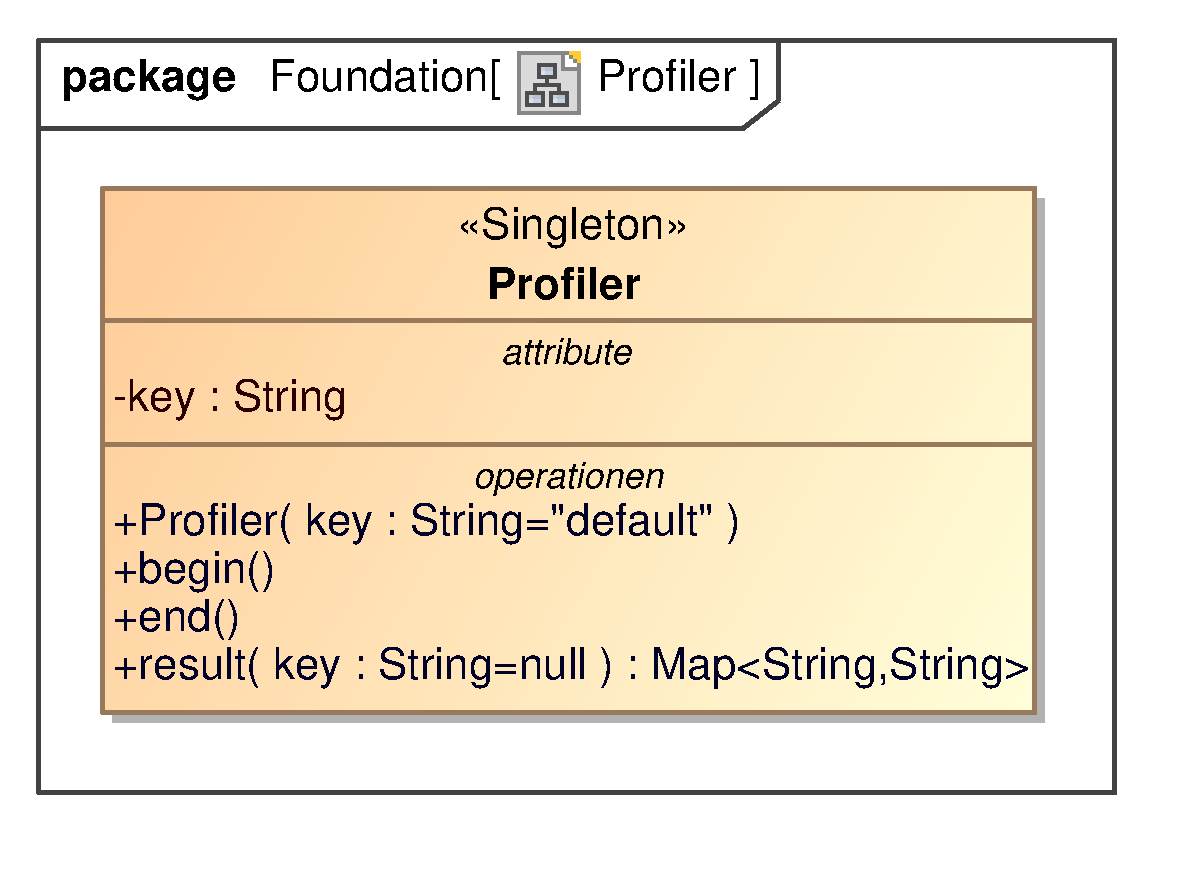
\includegraphics[width=0.75\textwidth]{gfx/MtGDeepAnalysis/Profiler.eps}
    \caption{Klassendiagramm Foundation.Profiler}
    \label{fig:class:foundation.profiler}
\end{figure}
%TODO: ...

%%%%%%%%%%%%%%%%%%%%%
%% Transformations %%
%%%%%%%%%%%%%%%%%%%%%
\subsubsection{Transformations.Cards}
Die Klasse \verb|Transformations.Cards| hat die folgenden Schnittstellen:

\begin{figure}[H]
    \myfloatalign
    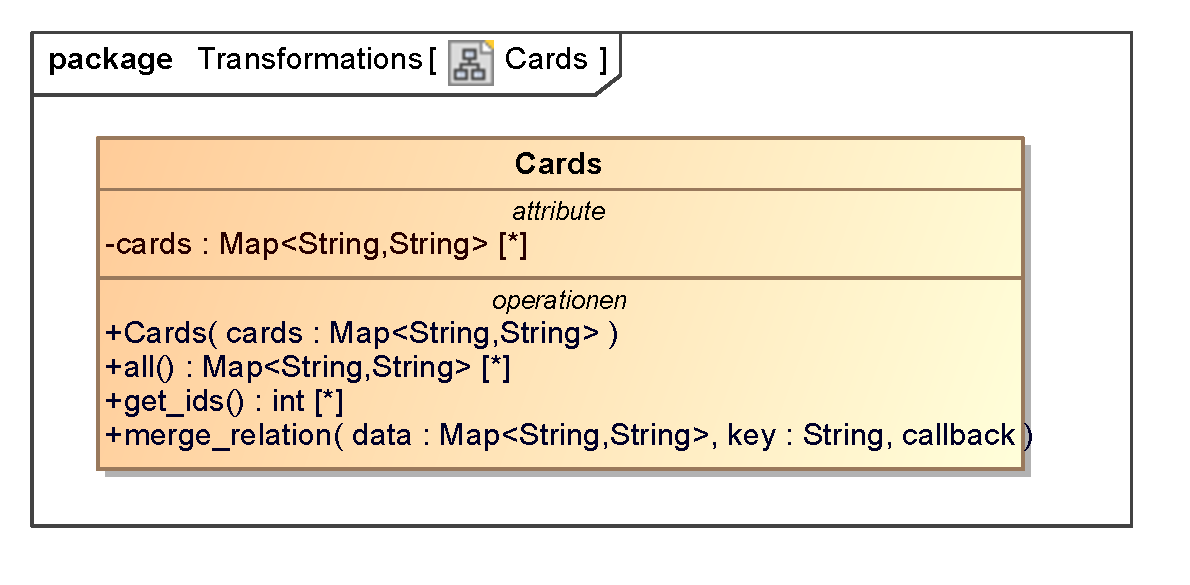
\includegraphics[width=0.75\textwidth]{gfx/MtGDeepAnalysis/Card_Transformations.eps}
    \caption{Klassendiagramm Transformations.Cards}
    \label{fig:class:transformations.cards}
\end{figure}

\begin{description}
    \item[constructor(cards)] \hfill \\
    Speichert Karten in \verb|cards|. Die Liste der Argumente befindet sich in \autoref{tab:transformations.cards.constructor}
    \item[all()] \hfill \\
       Ausgabe aller Karten
    \item[get\_ids()] \hfill \\
    Gibt eine List von allen Karten-IDs zurück.
    \item[merge\_relation(data, key, item\_callback)] \hfill \\
    Fügt die Daten einer Beziehung zu den Karten-Daten hinzu. Die Liste der Argumente befindet sich in \autoref{tab:transformations.cards.merge_relation}
\end{description}

\begin{table}[h]
    \caption{Transformations.Cards::constructor(cards : Dictionary[])} 
    \myfloatalign
    \begin{tabularx}{\textwidth}{lX}
        \toprule 
        \tableheadline{Eingabe} & \tableheadline{Beschreibung} \\ 
        \midrule 
        \verb|cards : Dictionary[]| & Zu bearbeitende Karten \\
        \bottomrule 
    \end{tabularx}
    \label{tab:transformations.cards.constructor}
\end{table}

\begin{table}[h]
    \caption{Transformations.Cards::merge\_relation(data : Dictionary[], key : string, item\_callback : Closure)} 
    \myfloatalign
    \begin{tabularx}{\textwidth}{lX}
        \toprule 
        \tableheadline{Eingabe} & \tableheadline{Beschreibung} \\ 
        \midrule 
        \verb|data : Dictionary[]| & Daten der Verknüpfung \\
        \verb|key : string| & Name unter dem die Verknüpfung in den Karten-Daten verfügbar sein soll \\
        \verb|item_callback : Closure| & Funktion, um Elemente der Verknpüfung zu bearbeiten bevor diese zu den Karten-Daten hinzugefügt werden \\
        \bottomrule 
    \end{tabularx}
    \label{tab:transformations.cards.merge_relation}
\end{table}


%%%%%%%%%%%
%% Tests %%
%%%%%%%%%%%
\subsubsection{Tests.AbstractTestCase}
Die Abstrakte Klasse \verb|Tests.AbstractTestCase| hat die folgenden Schnittstellen:

\begin{figure}[H]
    \myfloatalign
    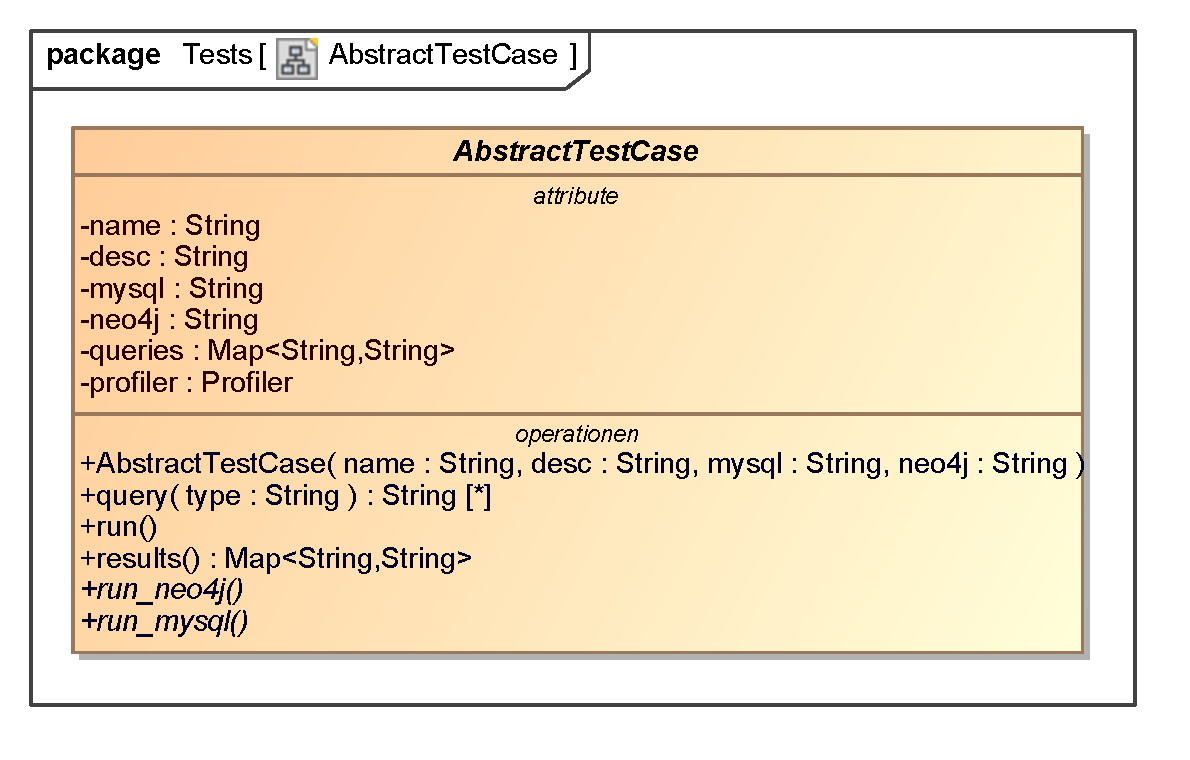
\includegraphics[width=\textwidth]{gfx/MtGDeepAnalysis/AbstractTestCase.eps}
    \caption{Klassendiagramm Tests.AbstractTestCase}
    \label{fig:class:tests.abstracttestcase}
\end{figure}

\begin{description}
    \item[constructor(name, desc, mysql, neo4j)] \hfill \\
    Setzt den Namen \verb|name| und die Beschreibung \verb|desc| des Testfalls. Außerdem werden die Schlüssel \verb|mysql| und \verb|neo4j| festgelegt, welche für die Testergebnisse benutzt werden.  Die Liste der Argumente befindet sich in \autoref{tab:tests.abstracttestcase.constructor}
    
    \item[query(type)] \hfill \\
    Gibt alle Abfragen für \verb|type = [mysql, neo4j]| die in dem Test ausgeführt werden zurück.
    
    \item[run()] \hfill \\
    Führt Test durch.
    
    \item[results()] \hfill \\
    Gibt aufgezeichnete Ergebnisse zurück nachdem der Test ausgeführt wurde.
    
    \item[run\_neo4j()] \hfill \\
    Testfall für Neo4j-Datenbank.
    
    \item[run\_mysql()] \hfill \\
    Testfall für MySQL-Datenbank.
\end{description}

\begin{table}[h]
    \caption{Tests.AbstractTestCase::constructor(name : string, desc : string, mysql : string, neo4j : string)} 
    \myfloatalign
    \begin{tabularx}{\textwidth}{lX}
        \toprule 
        \tableheadline{Eingabe} & \tableheadline{Beschreibung} \\ 
        \midrule 
        \verb|name : string| & Name des Testfalls \\
        \verb|desc : string| & Beschreibung des Testfalls \\
        \verb|mysql : string| & Schlüssel für MySQL-Testergebnisse \\
        \verb|neo4j : string| & Schlüssel für Neo4j-Testergebnisse \\
        \bottomrule 
    \end{tabularx}
    \label{tab:tests.abstracttestcase.constructor}
\end{table}

\subsubsection{Tests.Manager}
Die Klasse \verb|Tests.Manager| hat die folgenden Schnittstellen:

\begin{figure}[H]
    \myfloatalign
    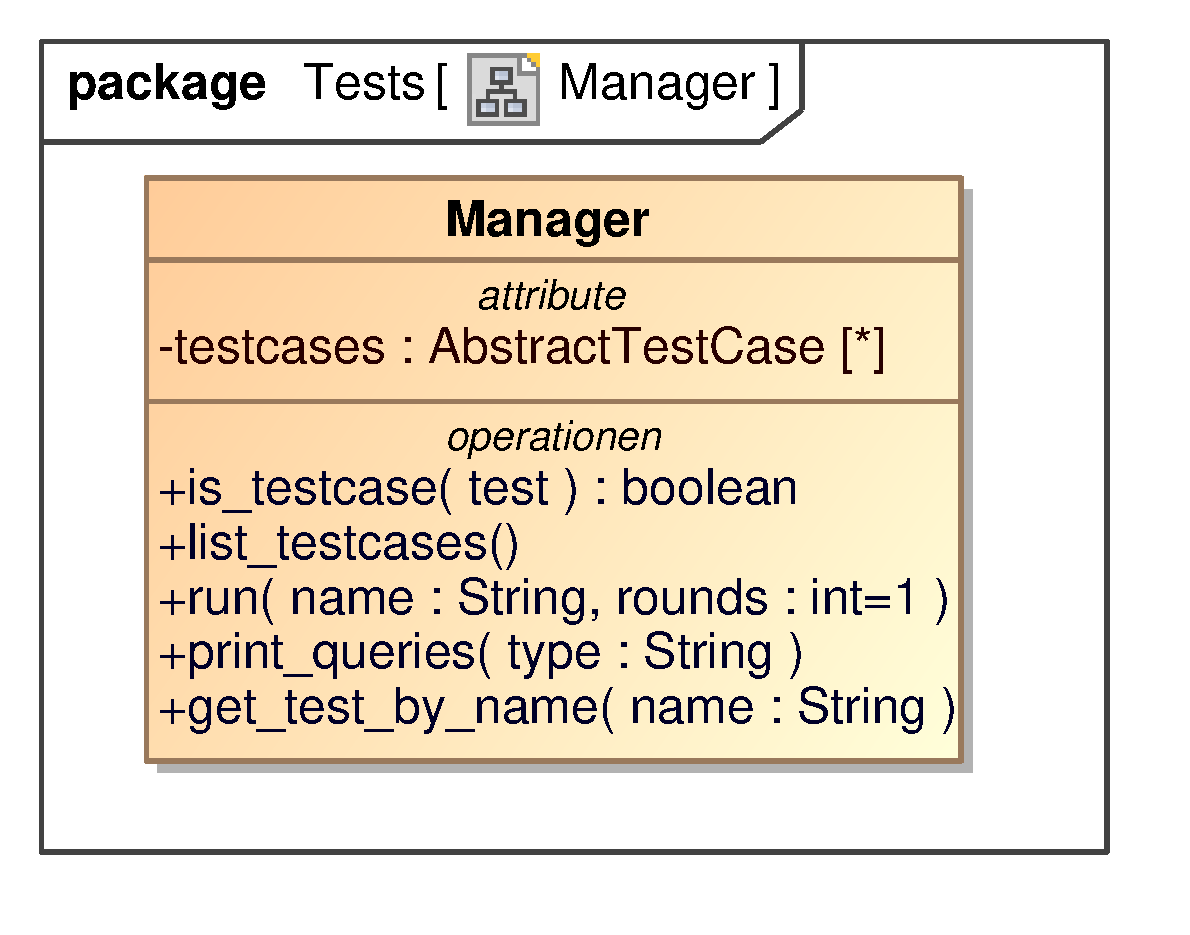
\includegraphics[width=0.75\textwidth]{gfx/MtGDeepAnalysis/Manager.eps}
    \caption{Klassendiagramm Tests.Manager}
    \label{fig:class:tests.manager}
\end{figure}

\begin{description}
    \item[constructor] \hfill \\
    Lädt alle Testfälle und speichert diese in \verb|testcases|
    
    \item[is\_testcase(test)] \hfill \\
    Prüft ob ein Objekt \verb|test| ein Testfall ist, das heißt von \verb|Tests.AbstractTestCase| abgeleitet ist.
    
    \item[list\_testcases()] \hfill \\
    Gibt eine Liste der verfügbaren Tests in \verb|testcases| aus
    
    \item[run(name, rounds)] \hfill \\
    Führt den Testfall \verb|name| \verb|rounds|-mal hintereinander aus
    
    \item[print\_queries(name)] \hfill \\
    Gibt alle Abfragen des Testfalls \verb|name| aus.
    
    \item[get\_test\_by\_name(name)] \hfill \\
    Gibt den Testfall \verb|name| zurück, sofern dieser sich in \verb|testcases| befindet
\end{description}

\begin{table}[h]
    \caption{Tests.Manager::constructor(name : string, desc : string, mysql : string, neo4j : string)} 
    \myfloatalign
    \begin{tabularx}{\textwidth}{lX}
        \toprule 
        \tableheadline{Eingabe} & \tableheadline{Beschreibung} \\ 
        \midrule 
        \verb|name : string| & Name des Testfalls \\
        \verb|desc : string| & Beschreibung des Testfalls \\
        \verb|mysql : string| & Schlüssel für MySQL-Testergebnisse \\
        \verb|neo4j : string| & Schlüssel für Neo4j-Testergebnisse \\
        \bottomrule 
    \end{tabularx}
    \label{tab:tests.manager.constructor}
\end{table}

\subsection{Schnittstellenrealisierung}
%
% Schnittstellenrealisierung -> Interaktionsdiagramm
%
\subsubsection{Fetch} %TODO: Change title
Fetch decks from mtgtop8.com \cite{mtgtop8} %TODO: Change description

\begin{figure}[H]
    \myfloatalign
    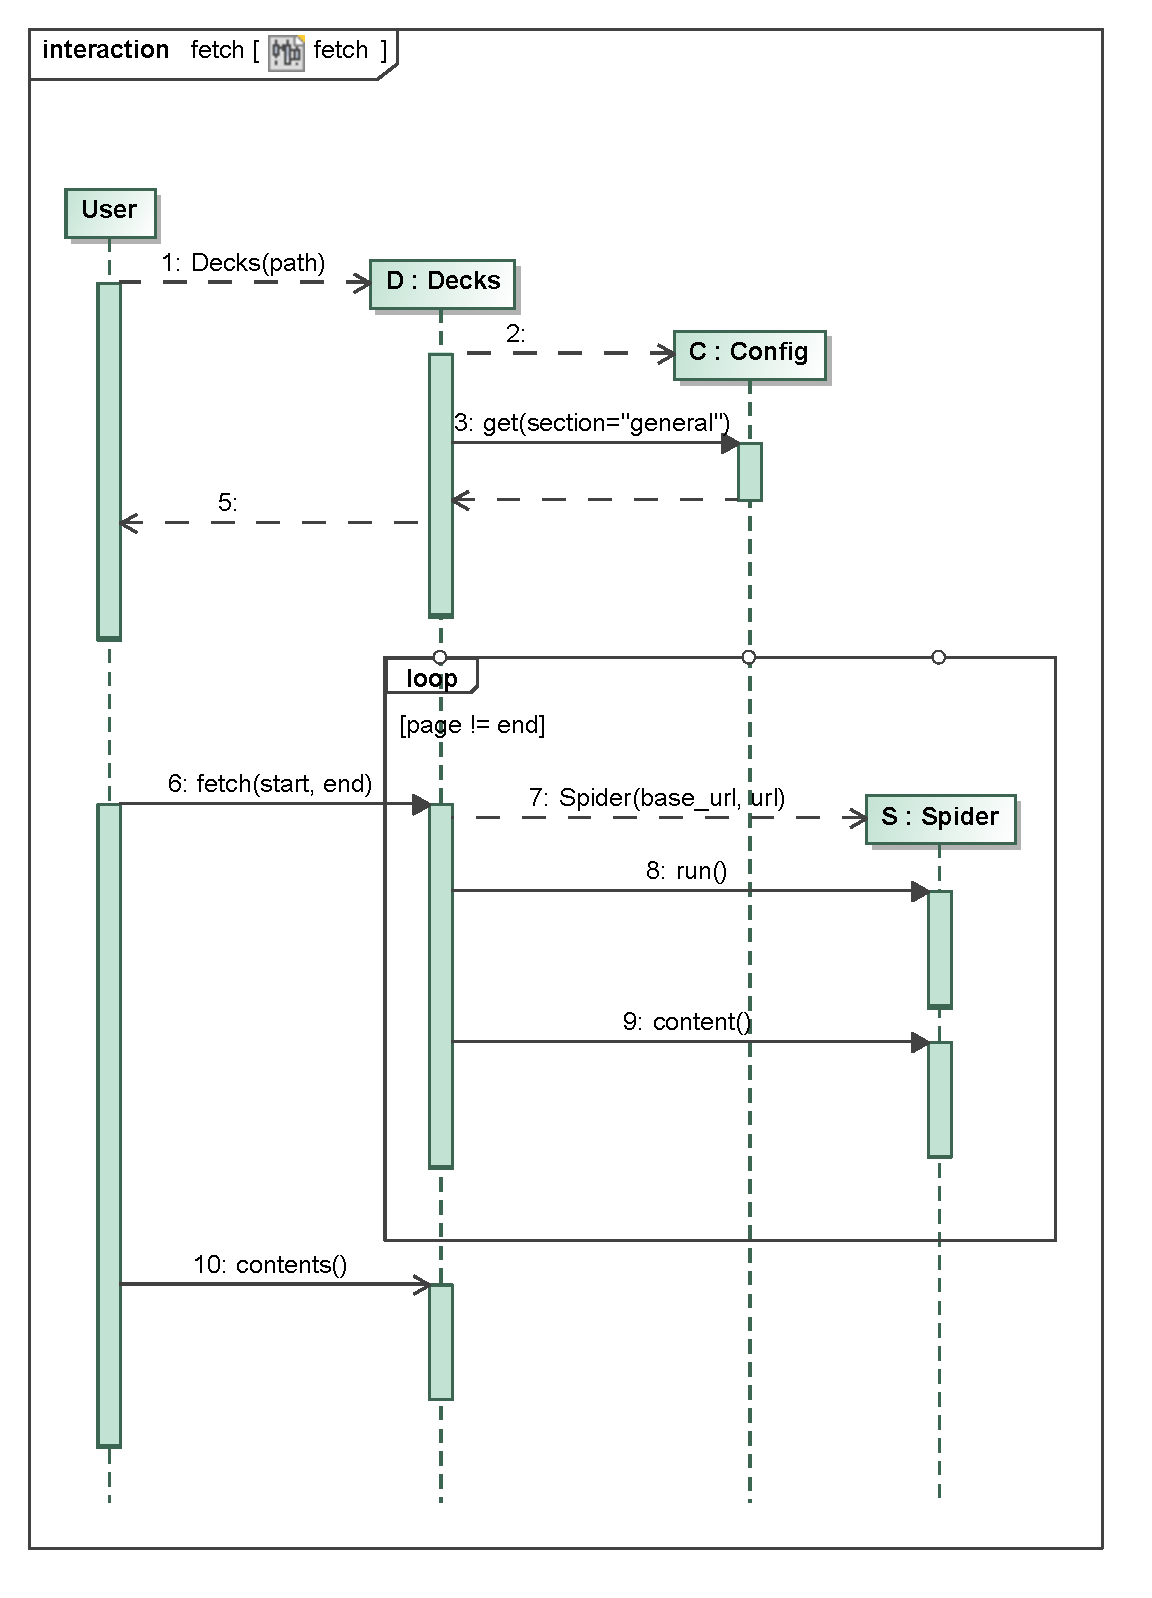
\includegraphics[width=\textwidth]{gfx/MtGDeepAnalysis/fetch.eps}
    \caption{Sequenzdiagramm Fetch} %TODO: Change caption
    \label{fig:seq:fetch}
\end{figure}

\subsubsection{Build} %TODO: Change title
Build \cite{mtgtop8} %TODO: Change description

\begin{figure}[H]
    \myfloatalign
    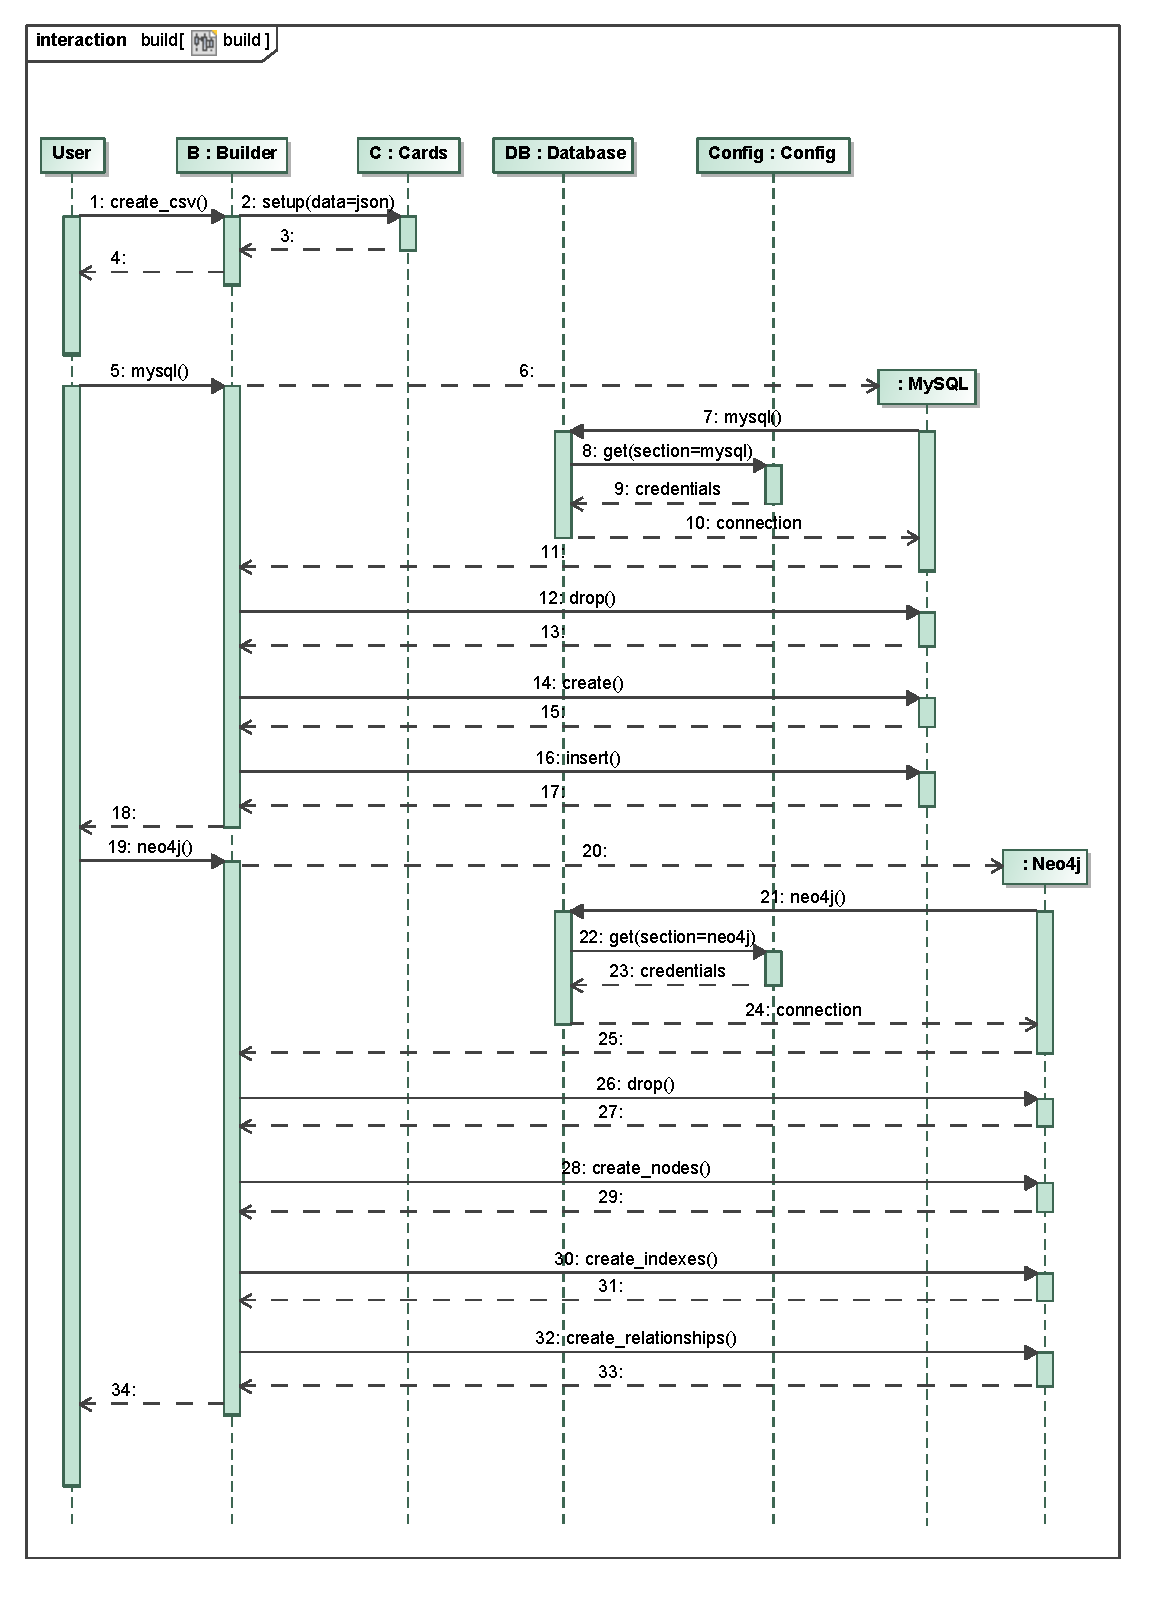
\includegraphics[width=\textwidth]{gfx/MtGDeepAnalysis/build.eps}
    \caption{Sequenzdiagramm build} %TODO: Change caption
    \label{fig:seq:build}
\end{figure}